\documentclass[]{report}

\usepackage{graphicx}
\usepackage{float}
\usepackage{caption}
\usepackage{multirow}
\usepackage{subcaption}
\setcounter{secnumdepth}{5}
\usepackage[margin=1.0in]{geometry}
\usepackage{appendix}


\title{Central Trigger Board FW Tests  \\ {\large Draft 0.1}}
\author{Jonathon Sensenig
	\\ \vspace{2em} University of Pennsylvania}
%\email{nfbarros@hep.upenn.edu}
%\thanks{Corresponding author}

\graphicspath{	{./figs//}}

\usepackage[final]{pdfpages}

\begin{document}
\maketitle

\tableofcontents

\chapter{}

The general idea is to go through and test iteratively the design adding the parts piece by piece. So the subsequent designs use the parts from previous design under the assumption they are tested and working.

\section{CTB Firmware Designs}

The design and testing evolution of the firmware for the CTB.

\subsection{Base Timing v3c}

The functionality is to generate timestamps from the timing endpoint and use the timestamp generator block to create a timing word every 
\textit{n} clock cycles. The words are sentoff to the processor side (PS) through a scatter-gather direct memory access (SG-DMA). 

This uses the older version 

	\begin{itemize}
		\item Nuno tested the SG-DMA part to $>$1MHz data throughput.
		\item The timing was verified to work by the timing words sent to the PS. They were
		monotonically increasing in increments of \textit{n} set by the timestamp generator block.
	\end{itemize}
 
\subsection{Base Timing v4a4}

Testing of the functionality of the timing endpoint. Mainly focusing on the connection between the CTB and timing board. The endpoint firmware itself is assumed to be fully functioning and tested by the University of Bristol, mainly Dave Newbold. 

	\begin{itemize}
		\item Verified the endpoint reaches the ready state (0x8) on CTB at CERN
			\begin{itemize}
				\item Read out timestamps
				\item Tested the START/STOP command. Correct flag on endpoint asserted/de-asserted.
			\end{itemize} 
	\end{itemize}
	
	\begin{itemize}
		\item Installed latest (v4a0) version of pdtbutler (software to control the timing system) at Penn
		\item Flashed the latest timing master firmware bitfile to timing board at Penn.
		\item Tested and received the same results on the CTB test stand at Penn as for the CTB at CERN.
	\end{itemize}

\subsection{Random Triggers}

The addition of random triggers. This is to allow a minimum bias trigger for the running of Protodune along with a test trigger data flow before the subsystems are connected to the CTB. In reality the minimum bias trigger might be handled by the timing board, but this is still TBD.

The major changes and additions are:

	\begin{itemize}
		\item Random trigger block:
			\subitem This block takes inputs from the triggers in the design. The idea is that whenever there are no triggers being generated the random triggers begin. If a trigger is generated the random trigger is disabled until a the trigger rate time has elapsed. The rate can be set via the config manager e.g., 10 = 10Hz. There is also a mask on the input triggers which allows one to set which triggers dictate whether or not a random trigger is allowed or disallowed. 
		\item Packet serializer block
			\subitem This is essentially a modified version of the packet sorter from the 35t experiment. It is much smaller since the firmware design only has 3 parallel sources of data, low level triggers (LLTs), high level triggers (HLTs), and timestamps. The FIFOs for these 3 sources are external to the block. The serializing happens by collecting the \textit{t$\_$valid} signals in a FIFO inside the block. If $>$1 sources produce a word simultaneously this is stored in the FIFO and then the words are read out of the external FIFOs accordingly ????(not exactly sure how). Otherwise, the words are simply read out, dropped into a FIFO synchronous to the PS clock (not sure this is necassary???) and passed to the DMA (actually they accumulate in a bundle before being sent to the DMA to increase throughput).
		\item Vivado supplied FIFOs per data word generator block, so 2 total. One for the timestamp generator one for the random trigger.
			\subitem AXI4-Stream Data FIFOs are included with the Vivado tool. Here is where the clock domain is crossed from the timing supplied 50MHz clock to the processor supplied 50MHz clock.
		\item Modification of the configuration manager
			\subitem Added an output to set the random trigger rate
			\subitem Added inputs for endpoint status, PLL lock
			\subitem Made the necessary changes in software to handle this. Mainly added an if statement to catch what I called the \textit{RandomTriggerFreq} (range: 1 - 50x1$0^6$) configuration and write it to a register.
	\end{itemize}
	
	\begin{itemize}
		\item[1.] Verified that I could still send data (timestamp words) with the new-ish packet serializer. 
		\item[2.] Verified that the random trigger was sending triggers, both the trigger word and the scalar trigger signal.
		\item[3.] Verified the block is sensitive to the trigger inputs by using the switches on the MicroZed carrier board. 
		\item[4.] Verified that I could send data from the timestamp generator and random trigger. So for random trigger at 50Hz and timestamp generator at 10Hz there are 5 trigger words for every timestamp word.
		\item[5.] Speed test up to 2 MHz (1kHz x 2kHz) without loss of words. However, this was with small FIFOs 1024 depth which should be increased.
	\end{itemize}

\subsection{Timing with returned Triggers}

The next step is to see if we can talk back to the timing board so we can eventually send triggers. The endpoint interface has 4 control signals (req, last, ack, ren) and a data line of which we are only allowed to use the 4 most significant bits.
	\begin{itemize}
		\item \textbf{req} Request to send a byte
		\item \textbf{last} Indicate the last byte is being sent
		\item \textbf{ack} Acknowledge the request to send a byte
		\item \textbf{ren} Indicates when the endpoint is ready for another byte
	\end{itemize}
	
I create a block to handle the sending of the data, asserting and deasserting the lines at the required times. The signals can be seen in the scope screenshot in Fig.\ref{fig:trigger_sigs}. Since in practice we only send a single byte at a time, the last signal is asserted immediately.

	 \begin{figure}[H]
	 	\centering
	 	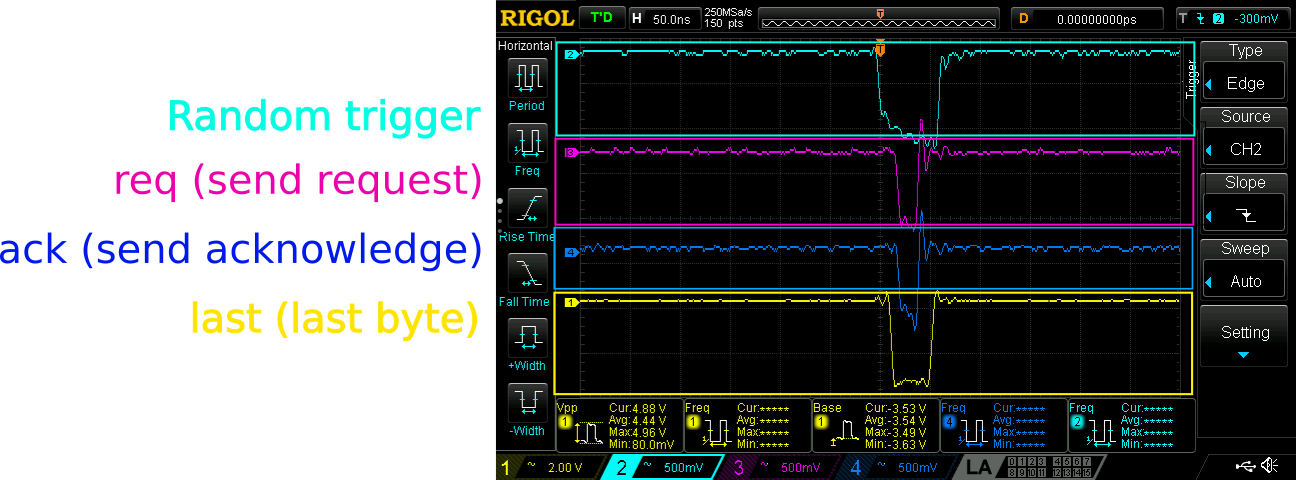
\includegraphics[width=6.25in]{trigger_return_edit.png}
	 	\caption{Signals from the block which interfaces with the timing endpoint to send triggers. Note: These are negative going logic signals.}
	 	\label{fig:trigger_sigs}
	 \end{figure}
	 
\subsection{Signal Shaping}

There is a relatively wide range of time in which signals can arrive from a subsystem to the CTB. This can be physics related such as the difference in time between the prompt and late light of LAr. We can stretch the pulse \textit{n} clock cycles to accommodate the difference so that a coincident window can still be formed.

	 \begin{figure}[H]
	 	\centering
	 	\includegraphics[width=5.25in]{signal_stretch_diff.png}
	 	\caption{(top) signal from pulse generator (middle) signal stretched by 1 clock cycle (bottom) signal stretched by 8 clock cycles.}
	 	\label{fig:pulse_shape}
	 \end{figure}
	 	 
	 	 
\section{Triggers}

This section will cover the testing of the triggers for the various subsystems.

\subsection{Beam Triggers}

The beam trigger is largely dependent on having all of instrumentation fire in the event there is a particle of interest, i.e., as the particle travels along the length of the beam line. Thus we will start with an inclusive trigger.

\subsubsection{Trigger 0}

We will start with defining the inputs, arbitrarily.

	 \begin{figure}[H]
	 	\centering
	 	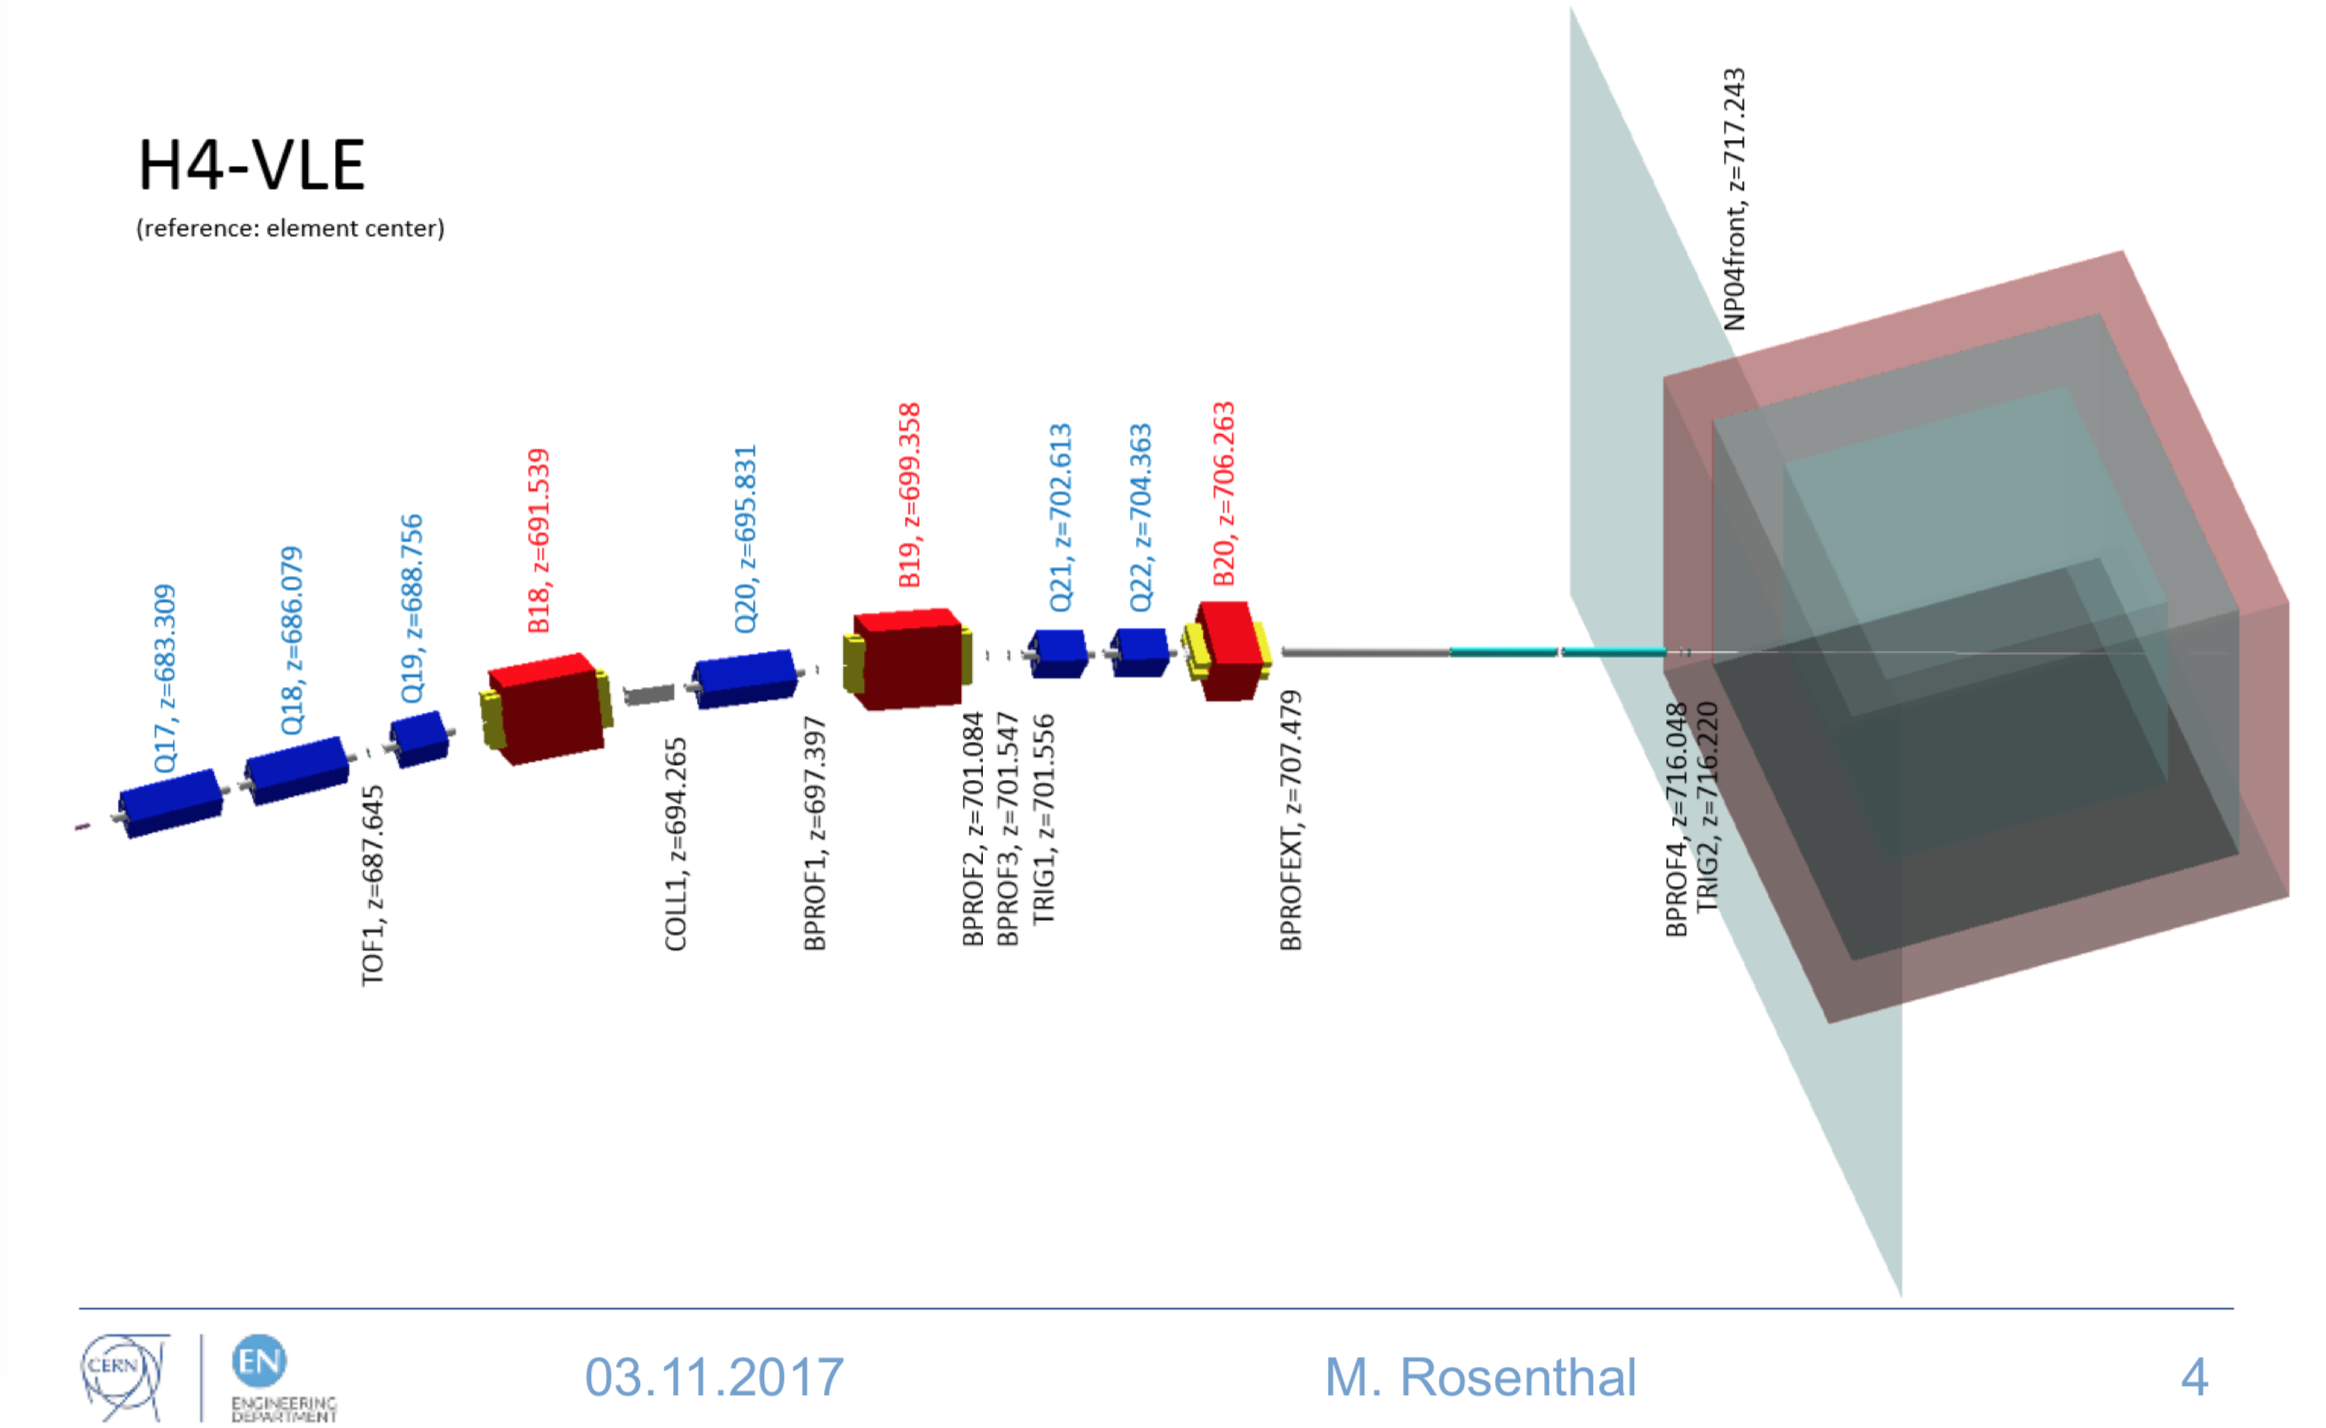
\includegraphics[width=5.25in]{h4beam.png}
	 	\caption{Beamline instrumentation.}
	 	\label{fig:h4beam}
	 \end{figure}

\begin{itemize}
	\item[\textbf{1}] Beam gate
	\item[\textbf{2-6}] Scintillating fiber (Sci-Fi) beam profile monitors 1-5
	\item[\textbf{7}] Time of Flight (ToF) 1 and 2 
	\item[\textbf{8-9}] Cherenkov detectors 1 and 2
\end{itemize}

The inclusive mask will be such that all the detectors except the one Cherenkov detector.

\begin{center}
	mask$_{inc}$ = [8:0] = 011111111
\end{center}

\subsection{CRT Triggers}

The CRT will probably use 35t style triggers.

	 \begin{figure}[H]
	 	\centering
	 	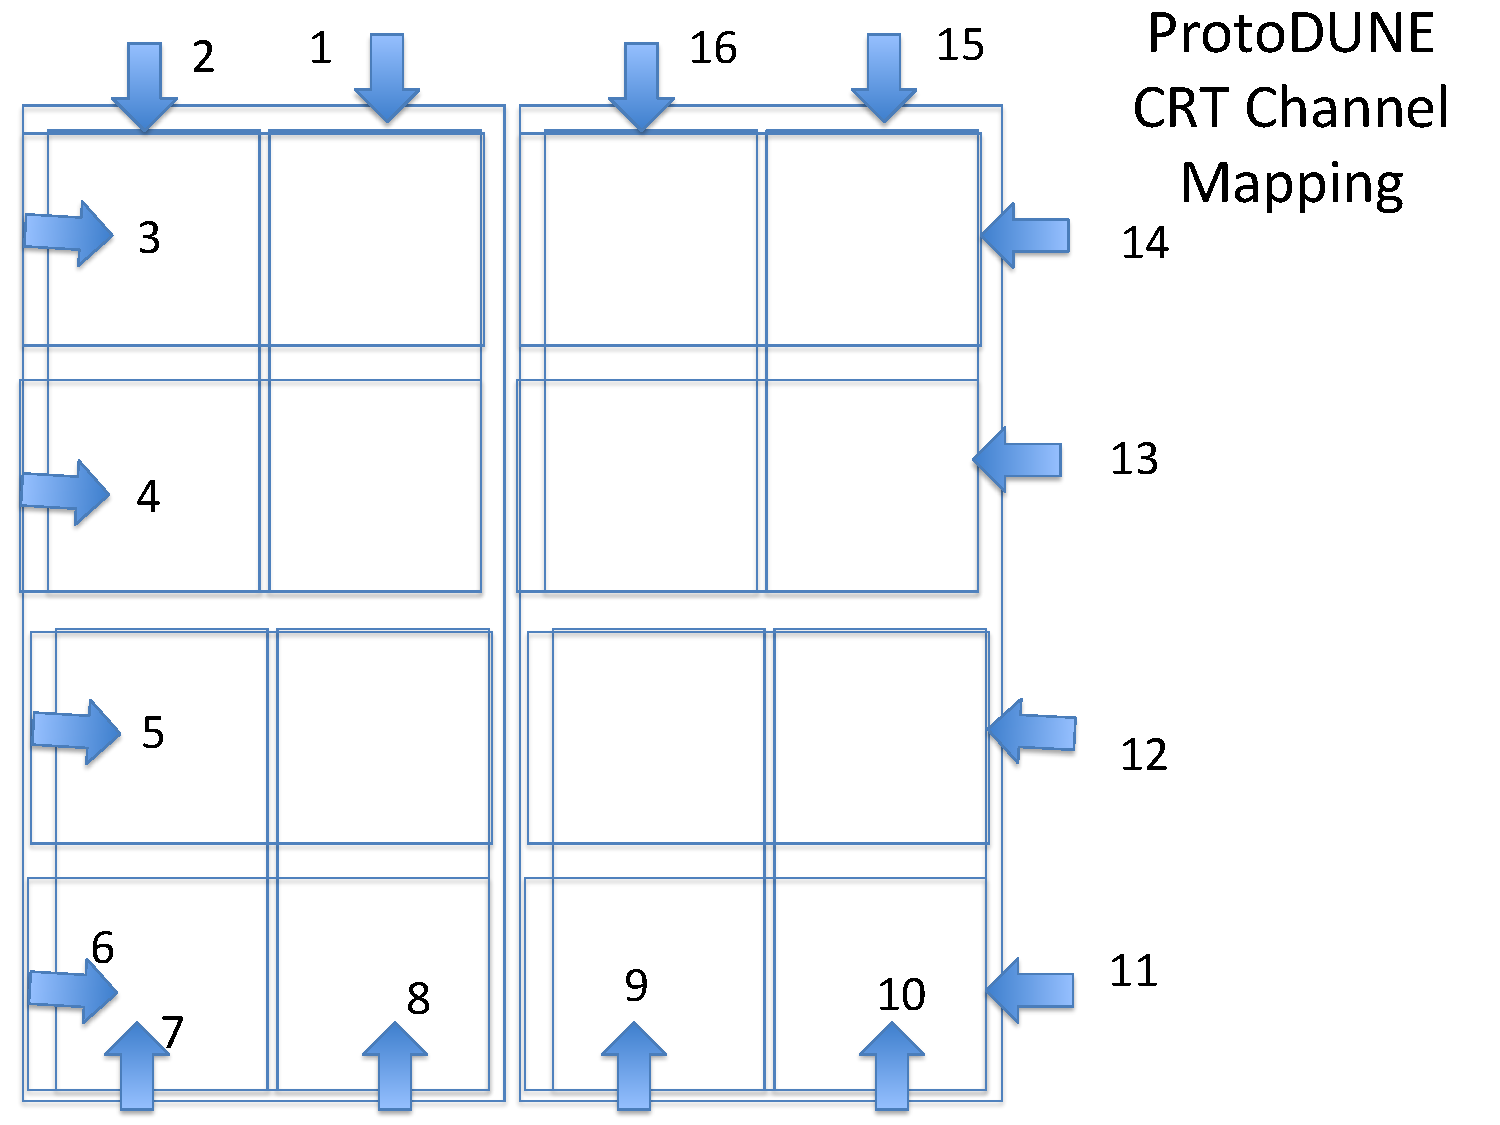
\includegraphics[width=5.25in]{crt_mapping.pdf}
	 	\caption{Mapping of the CRT channels.}
	 	\label{fig:crt_ch_map}
	 \end{figure}

\subsubsection{Trigger 0}

Any TPC crossing cosmic particle. In other words a hit on both plains on one side of the cryostat followed (practically instantly) by a signal from both planes on the opposite side.

\subsection{PDS Triggers}

The PDS will most likely be used with a counting trigger, i.e., there are greater than X PDS triggers, therefore a trigger is issued. A possible inclusive mask trigger is for the beam, as the events will be constrained mostly to 1-3 TPCs.

\subsubsection{Trigger 0}

\begin{appendices}
	\chapter{ Test Vectors}
	
	\begin{center}
		%make table here
		\textbf{vv} 00110010
		
		\begin{table}[ht]	
		\caption{Nonlinear Model Results}% title of Table
		\centering % used for centering table
		\begin{tabular}{c c c c}	% centered columns (4 columns)
		\hline \hline                %inserts double horizontal lines
		Case & Method\#1 & Method\#2 & Method\#3 \\ [0.5ex] % inserts table 
		%heading
		\hline % inserts single horizontal line
		1 & 50 & 837 & 970  \\	% inserting body of the table
		2 & 47 & 877 & 230  \\
		3 & 31 & 25  & 415  \\
		4 & 35 & 144 & 2356 \\
		5 & 45 & 300 & 556 \\ [1ex]	% [1ex] adds vertical space
		\hline	%inserts single line
		\end{tabular}
		\label{table:nonlin}	% is used to refer this table in the text
		\end{table}
		
	\end{center}
\end{appendices}
	 	 
\end{document}